\documentclass[a4paper, doc, draftall]{apa6}
\usepackage[american]{babel}
\usepackage[backend=biber,style=apa]{biblatex}
\DeclareLanguageMapping{american}{american-apa}
\addbibresource{references.bib}
\usepackage{amsmath,amssymb,amsfonts}
\usepackage{algorithmic}

\usepackage[utf8]{inputenc}
\usepackage{amsmath}
\usepackage{graphicx}
\usepackage[colorinlistoftodos]{todonotes}
\usepackage{lineno}
\usepackage{widetable}
\usepackage{eurosym}
\usepackage{minted}
\usepackage[toc,page]{appendix}
\usepackage{todonotes}

\addbibresource{references}

\linenumbers


\title{Misjudging distances between shifted curvy lines in comparison to straight lines}
\shorttitle{Misjudging distances between \dots}
\author{Marc Weitz}
\affiliation{Department of Psychology\\University of Tuebingen}

\authornote{
	Correspondence concerning this article should be addressed to Marc Weitz, E-mail: marc-stephan.weitz@student.uni-tuebingen.de . This report is also available at \url{https://osf.io/x7ha9/}.
}


\abstract{
	Visual perspective is an important part of cognitive psychology and computer vision. It investigates the question in which way objects appear to the eye based on their spatial attributes or their dimensions and the position of the eye relative to the objects. Many studies have shown that what we perceive is not necessarily what there is in the physical domain.\\
	In this expose we propose an experiment such a difference between the cognitive and the physical domain in the perception of lines. The goal of our study is to show that is unequally more difficult to humans to decide whether a line is shifted in one direction for non-linear, e.g curvy lines, that for linear, e.g. straight, lines.\\
	By freely adjusting a line, untill it appears to the participants that it is shifted to another reference line, we will messeaure the misjudment for three different straight or curvy lines. We expect a good judgement for the  straight line and a significant misjudgement for the curvy lines. Moreover, we expect this misjudgement to be larger, the more curvy the lines are.\\
}

\begin{document}
\maketitle


\section{Current state of research}

The question how we perceive the world has been intensively studied by cognitive psychologists for decades. In the last years, with growing computational power and advances in the field of computer vision, the question became more and more relevant.\\
A wide range of experiments showed that what humans perceive is in many aspects significantly different from what is out there in the physical domain. Although, this holds also for other domains than the visual domain, the visual domain is of particular interest as understanding how we perceive the world can substantially help us to create better renderings in computer vision or to design better usable interfaces for a wide range of tasks.\\
Therefore, especially the study of perspective is of interest. This field has been studied by scientists as well as artists for centuries. In arts using one or more vanishing points became popular to introduce a third dimension of depths to an two dimensional image. In this kind of perspective drawing parallel lines in the physical domain are directed to a vanishing point in the picture. For example, the parallel lines of a railway track are perceived by a standing human being as meeting at a distant point at the horizon.\\
In the effect we are aiming to describe, we face a similar but still different situation where the lines are drawn in parallel in the picture space. Thereby, the parallelism is defined as a shift in one direction. However, introspectively the lines do not seem to be shifted in one direction. Instead, the distances between the lines seem to vary along the other dimension.\\
In this expose we propose an experiment to properly describe this effect. Therefore, we propose an experiment, where the participants have to adjust one line to another reference line. The participants get instructed that they should adjust the line in a way so that it always has the same distance to the other line at any point.\\
However, we assume that this experiment might be very exhausting with many trials and also it is very likely that the participants quickly get the intention of the experiment. As this would question the nativity of the participants, we will perform this experiment on Amazon's Mechanical Turk (MTurk), a popular crowd-sourcing labor market. MTurk is run by the well known marketplace Amazon and offers the opportunity of inexpensive but still high-quality data \parencite{buhrmeister2011}. Thereby, MTurk provides further advantages. \\
Firstly, participants recruited by this method are slightly more demographically diverse than other standard Internet samples and are significantly more diverse than typical college samples \parencite{buhrmeister2011}. These samples of Western, Educated, Industrialized, Rich and Democratic (WEIRD) are predominant in psychological research and may be partly responsible for the replication crisis.\\ % TODO citation needed
Secondly, the obtained data is as reliable as those obtained via traditional methods \parencite{Hilbig2016, deLeeuw2016, paolacci2010}. It is notable, that data collected by Amazon's Mechanical Turk costs only less than half than traditionally collected data as the investigator has to compensate the participant as well as a conductor.\\
Nevertheless, not all experiments can be delivered online \parencite{gosling2010advanced}. For obvious reasons EEG or other methods requiring a special setup are restricted to be performed in a laboratory. However, especially behavioural experiments but also psychophysical experiments might be conductible on Amazon's Mechanical Turk \parencite{Mason2012, paolacci2010}.\\
We expect our experiment to perform well on Amazon's Mechanical Turk. Especially due to the small number of trials of each participant, MTurk has a large advantage over laboratory based research. Moreover, the data we are aiming to collect is mostly hardware independent as we only collect the adjustment which should be not infected by the setup of the participant. 

\section{Proposed Method}
	The projects aims to full fill the standards of open science and will be preregistered at \url{https://osf.io/}. All materials, data and analysis will be published there and respectively in a repository on GitHub. All materials and software used to conduct in this experiment are therefore free, publicly available and open source.
	
	\subsection{Sample}
		The participants will be divided into three groups of XX participants each. All participants have to consent that they are full-aged. However, the reported demographics of MTurk users under 18 years of age are very low \parencite{Mason2012}. Nevertheless, it can not be fully guaranteed that all participants are full-aged. Furthermore, the participants have to consent to have normal or corrected-to-normal vision.
		
		\subsubsection{Risks, debriefing and informed consent}
			The risks of mental or physical impairment are estimated to be relatively low. As the experiment for each participant only consists of one trial, we do not expect that there will be a necessity for breaks. However, all participants will be informed that they are allowed to pause or quit the experiment at any point.\\
			All participants will be informed of the risks and requirements with a written statement prior to the experiment to which they have to consent to. In this step, the participants also have to provide demographical features such as age and gender.\\
			As the experiment is not conducted in a classical laboratory, the data has to be transmitted through the internet. As the data contain potentially sensitive data, the transmission to the server where the experiment is hosted has to be encrypted using the SSL standard.\\
			All participants will be shortly debriefed after the experiment, describing the purpose of the experiment and providing information on how to contact us in event of questions or complaints. 
	
	\subsection{Material}
	\begin{figure}[!t]
		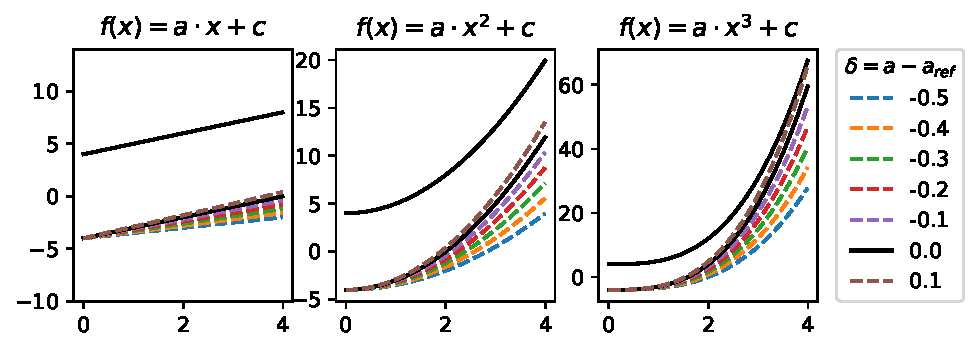
\includegraphics[width=\textwidth]{plots/examples.pdf}
		\caption{Example lines of the polynomials $x, x^2$ and $x^3$. The reference polynomial (upper black line) is shifted 8 units in $y$-direction. The dotted coloured lines represent different values of $a$ and are shown as the difference $\delta$ from the reference value $a_{ref}$.}
		\label{examples}
	\end{figure}
	\subsubsection{Client-side}
	Each trial consists of two polynomials shifted along the y-axis. One of the polynomials is the reference to where the other polynomial has to be adjusted to. Examples of this setup are shown in Figure~\ref{examples}.\\
	The experiment will be programmed with javascript, a client side web programming language. An example web experiment\footnote{\url{https://github.com/feste/experiment_template}} using javascript is for example provided by the Computation and Cognition Lab of the university of Stanford\footnote{\url{https://cocolab.stanford.edu/}}.\\
	\subsubsection{Server-side}
	The experiment has to be hosted on publicly available server. The deployment of the software for this server can be done using Psiturk \parencite{mcdonnell2012psiturk}. Psiturk is a Python3 based application to run and host psychological experiments for Mechanical Turk \parencite{Gureckis2016}. It uses the Python micro web framework Flask \parencite{ronacher2010flask} and provides functionality to deploy and to publish experiments on Amazon's Mechanical Turk.
		
	\subsection{Procedure}	
		\subsubsection{General procedure}
			The participants will be welcomed and informed about possible risks, the procedure of the experiment and the possibility to pause or quit the experiment at any time. This information will be provided prompted on the computer screen where the participants have to consent that they have read, understand and agreed on these terms. Furthermore, the participants have to state that they are over the legal age of 18 years.\\
			Afterwards, the participants perform the experiment. The participants are free to pause the experiment at any time, even though the experiment only consists of one trial.\\
			Finally, the participant will be debriefed at another info screen after the experiment, describing the purpose of the experiment and providing information on how to contact us in event of questions or complaints.\\
			The participation in the experiment will be compensated with 0.04 \euro per trial, which is a usual rate for tasks on Amazon's Mechanical Turk.
		
		\subsubsection{Experimental procedure}
			After consenting to the terms of use a screen will be shown with the instructions for the experiment. Afterwards a short screen showing a fixation cross at the centre of the screen is used to standardise vocal point.\\
			Centred on this point, two lines are shown in the next step. Depending on the group, the participants are assigned to, the lines are different, but all following the structure of 
			$$ f(x) = a \cdot x^b + c $$
			where $b$ is manipulated between the groups.\\
			The task of the participant is to adjust one of the lines in the way that the participant perceives the two lines to be equidistant in y-direction at any point. This adjustment can be done freely using two keys %todo Should the keys and step size already be specified
			on the keyboard changing the parameter $a$ in small steps. The keys are the same for all participants.\\ 
			After adjusting the line, the participant has to confirm his input by pressing the space key. The input together with the demographical information of the participant will be directly transmitted and stored on the hosting server.
			
	\subsection{Variables, Hypothesis and Analysis}
		\subsubsection{Variables}
			As our independent variable we manipulate the polynomial's degree which corresponds to larger gradients for larger polynomial's degrees. This respectively also refers to the curviness of the line.\\
			Furthermore, we manipulate the starting value of $a_b$ of the polynomial which should be adjusted by the participant. $b$ thereby describes the degree of the polynomial and respectively the assigned group. This is to ensure our measurements are not just a result of starting position bias.\\			
			As a dependent variable we measure the participants' estimate of $a_b$: $\hat{a}_b$. To make the estimates in the different groups comparable we, use the affine-linear transformation of calculating the deviation $\delta$ of the measured value $\hat{a}_b$ from the correct value $a_b$, defined as
			$$\delta_b = \hat{a}_b - a_b$$
			
		\subsubsection{Hypothesis}
			\begin{figure}
				\centering
				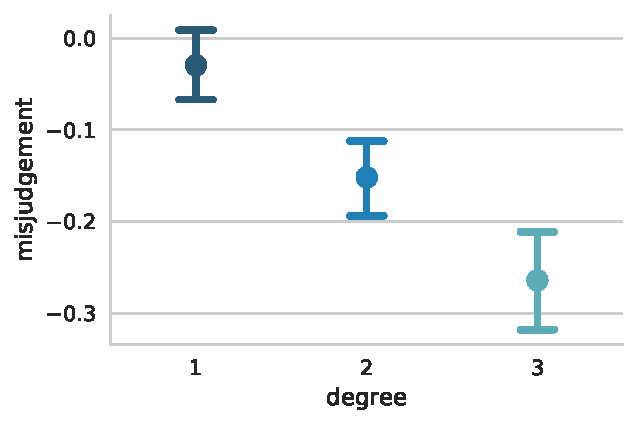
\includegraphics[width=0.6\linewidth]{plots/results.pdf}
				\caption{Expected main effect for the polynomial degree. The misjudgement is expected to increase (in negative direction) with a larger slope of the line.}
				\label{results}
			\end{figure}
			We expect a misjudgement of the distances for curvy lines but not for the straight line. Furthermore, we expect a larger misjudgement the larger the gradient respectively the curvature of the reference line becomes. The expected result pattern in shown in Figure~\ref{results}.\\
			As the gradient of a polynomial increases with increasing degree, we expect $\delta_x < \delta_y < \delta_z$ for $x < y < z$ which leads to the linear Nullhypothesis 
			$$H_0: \delta_x = \delta_y = \delta_z$$
		
		\subsubsection{Analysis}
			The linear Nullhypothesis described above can simply be tested with a one-way ANOVA. However, as we expect larger values for curvier lines, we might lack on homoscedasticity, wherefore we might need to encounter by transforming the data.\\
			Furthermore, we expect the deviation $delta_b$ to be significantly different from zero already for small values of $b > 1$. For $b = 0$ or $b = 1$ (if the curve is a straight line) we expect the deviation to be not significantly different from $0$.\\
			Contrarily, different starting points should have no influence on the estimate of $a$. This will be tested using a nested model comparison using a Likelihoodratio test. Thereby, we compare the model including the starting points with the one not including them. The model not including the starting points is thereby the same as we use for the analysis of variance to test whether their is a significant difference in the estimates. 
	
\section{Schedule}

The experiment can be created and conducted by one person. All required software is released under open source licenses and can easily and be downloaded from the internet at no charge. The proposed schedule is shown in Table~\ref{schedule}.\\
As this experiment is planned to be open science all steps might require more time than closed science experiments since all steps are publicly visible and therefore need special care.\\
We estimate the required time to be circa 12-13 weeks. Thereby, collecting the data (4 weeks) and writing the final report (4 weeks) are the most time consuming steps. Due to the bright range of examples and software provided by the open science community, we expect the programming of the experimental software to be done quickly. However, as conducting experiments on Amazon's Mechanical Turk is a relatively new method in psychological science, we may encounter some unexpected problems.


\begin{table}[t!]
	\caption{Proposed schedule to create and conduct the proposed experiment as well as a specification of the costs.}
	\label{schedule}
\noindent
	\begin{tabular}{*{4}{l}} 
		\centering
		Task & Requirements & Costs & Required time\\
		\hline
		Progamming the experimental software & JavaScript, Docker & 0 \euro & 2-3 weeks\\
		Production testing & Server & ? & 1 week\\
		Create session files & Python & 0 \euro & 1 day\\
		Create analysis script & R or Python & 0 \euro & 1 day \\
		Preregistration at \url{osf.io} & & 0 \euro & 1 day\\
		Collect data & Server, ? & ? & 4 weeks\\
		Data analysis & R or Python & 0 \euro & 1 day\\
		Writing the report & \LaTeX & 0 \euro & 4 weeks\\		
		\hline
		Overall: & & & 12-13 weeks\\
		
	\end{tabular}
	
	All steps require a Computer with an installed 64bit Linux operating system. The server should also have a 64bit Linux OS installed and should be accessible via a DNS entry under a certain domain. The required software (JavaScript, Docker, R, Python and \LaTeX) are all Open Source and free to use. \\
	The required timings are sometimes overlapping and the 12-13 weeks therefore represent an upper bound.
\end{table}

\section{Outlook}
	In the proposed experiment we are aiming to examine the perception of lines. Our goal is to formal describe the presented optical illusion. Therefore, the participants have to freely adjust a line to the point where they perceive the line to be equidistant to another reference line. We expect a significant difference in the judgement for curved lines compared to straight lines. Moreover, we expect this effect to be larger the curvier a line is and to not exist for straight lines.\\
	However, even tough we can confirm a relation between the curviness of the line and our misjudgement of the distances, the nature of this relation remains unknown. Further research is necessary to examine this relationship.\\
	To quantify this relation we propose an experiment with more levels of the factor polynomial degree/gradient. Then, a generalized additive model \parencite{wood2006generalized}, short GAM, could be fitted with a spline for the factor of curviness. The large penalisation of the basis functions which construct the spline in a GAM enables to sufficiently detect non-liner relationships without the tendency to over-fit the data.\\
	Moreover, it is necessary to integrate the possible effect into our current knowledge if we can confirm it. We especially see a potential connection to the perception of space. As it seems to us, that the distance between two curvy lines is underestimated if the slope is large, our brain might interpret the scene spatially. Therefore, similar to the parallel lines of a railway track, which are perspectively drawn to meet somewhere at the horizon, our brain might also add something like depth to this image.\\
	Investigating this effect can contribute to our understanding of perspective and perception in general. Perspective and how to add a third dimension of depth to images has a long history in arts. But also in new contexts like rendering 3D scenes in computer vision understanding how we spatially perceive the world is from particular interest. The research proposed in this expose therefore might contribute to more realistic renderings.\\
	But also for the usability and human computer interaction this might be of interest. Especially graphical designer often have to deal with aligning lines, straight as well as curvy ones. Understanding how we perceive and why we misjudge distances between lines can help to raise awareness as well as to design better computer programs which encounter the problem.\\
	As to the current state of knowledge of the authors there are no similar studies reported in the literature, the proposed experiment could build the basis of a new aspect of spatial cognition. However, much effort is required to further understand the described effect and to put it in relation to other aspects of cognitions and perception.
	
	


\printbibliography
\newpage

\begin{appendices}
	\section{Source code for the plots}
		\subsection{plots/examples.py}
		\label{code:examples}
		\inputminted[mathescape, linenos, numbersep=5pt, frame=lines, framesep=2mm]{python}{scripts/examples.py}
		\newpage
		
		\subsection{plots/results.py}
		\label{code:results}
		\inputminted[mathescape, linenos, numbersep=5pt, frame=lines, framesep=2mm]{python}{scripts/results.py}
\end{appendices}

\end{document}